\begin{center}
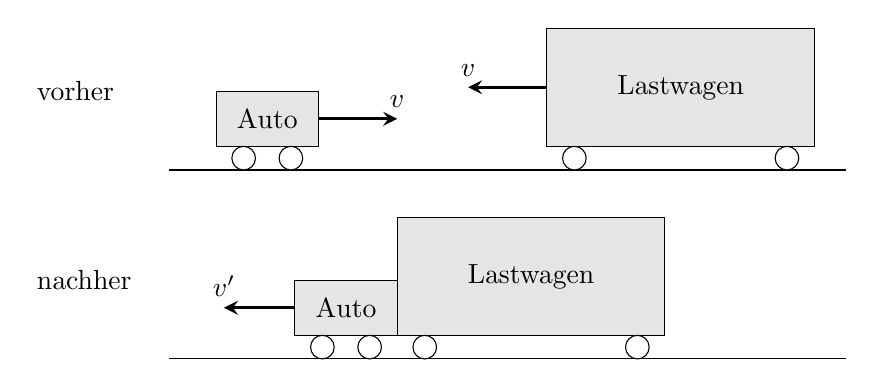
\begin{tikzpicture}[>=stealth]
 \node[anchor=west] at (0,1) {vorher};
 \draw (1.8,0) -- (10.4,0);
 \draw[fill=gray!20] (2.4,0.3) rectangle (3.7,1);
 \node at (3.05,0.65) {Auto};
 \draw[fill=white] (2.75,0.15) circle (0.15) (3.35,0.15) circle (0.15);
 \draw[->, very thick] (3.7,0.65) -- (4.7,0.65) node[above] {$v$};
 \draw[fill=gray!20] (6.6,0.3) rectangle (10,1.8);
 \node at (8.3,1.05) {Lastwagen};
 \draw[fill=white] (6.95,0.15) circle (0.15) (9.65,0.15) circle (0.15);
 \draw[->, very thick] (6.6,1.05) -- (5.6,1.05) node[above] {$v$};
 \node[anchor=west] at (0,-1.4) {nachher};
 \draw (1.8,-2.4) -- (10.4,-2.4);
 \draw[fill=gray!20] (3.4,-2.1) rectangle (4.7,-1.4);
 \node at (4.05,-1.75) {Auto};
 \draw[fill=white] (3.75,-2.25) circle (0.15) (4.35,-2.25) circle (0.15);
 \draw[fill=gray!20] (4.7,-2.1) rectangle (8.1,-0.6);
 \node at (6.4,-1.35) {Lastwagen};
 \draw[fill=white] (5.05,-2.25) circle (0.15) (7.75,-2.25) circle (0.15);
 \draw[->, very thick] (3.4,-1.75) -- (2.5,-1.75) node[above] {$v'$};
\end{tikzpicture}
\end{center}

Die Fahrtrichtung des Lastwagens ist positiv. Vor dem Stoss hat der Lastwagen die Geschwindigkeit $+v$, das Auto $-v$; danach bewegen sich beide gemeinsam mit $v'$. Impulserhaltung:
\begin{align}
 m_\text{L}\,v - m_\text{A}\,v &= \left(m_\text{A}+m_\text{L}\right)v'
\end{align}
Damit ist
\begin{align}
 v' &= \vEnF \\
   &= \frac{\left(\mLw-\mAu\right)\cdot\vCr}{\mAu+\mLw} \\
   &= \vEn = \vEnk \approx \result{\vEnkP{0}{3}}
\end{align}
Die beiden Fahrzeuge bewegen sich in der ursprünglichen Fahrtrichtung des Lastwagens weiter; das Auto wird also mit hoher Geschwindigkeit zurückgeschoben.
